\chapter{Anforderungen}

(Joshua)

In diesem Kapitel sollen die Anforderungen an die zu erstellende Applikation beschrieben werden, um den zu erreichenden Scope festzulegen und eine abschließende Bewertung durchführen zu können, die das Erreichte mit den Zielen vergleicht.

\vspace{0.25cm}

Zuerst wird die Begrifflichkeit \enquote{Anforderung} geklärt. In der Softwareentwicklung gibt es einige verschiedene Definitionen von \enquote{Anforderungen}. In dieser Arbeit soll der Definition gefolgt werden, welche von Helmut Balzert in seinem Buch zu den Basiskonzepten und des Requirements Engineering erarbeitet wurden \cite{Balzert.2009}. In seinem Werk werden Anforderungen wie folgt definiert.

\begin{defStrich}[Anforderungen]
	\enquote{Anforderungen (requirements) legen fest, was man von einem Definition
		Softwaresystem als Eigenschaften erwartet.} Mit der Annahme, dass \enquote{man} alle Stakeholder (Personen, die ein Interesse an der Entwicklung und/oder der erstellten Software haben) beinhaltet. \cite{Balzert.2009}
\end{defStrich} 

Des Weiteren sollten vor der Festlegung der Anforderungen \enquote{Visionen und Ziele} und die Rahmenbedingungen, in denen die Software existieren sollen, festgelegt werden. Erst danach sollten Eigenschaften, welche in \enquote{funktionale} und \enquote{nichtfunktionale} Eigenschaften unterteilt werden können, definiert werden. In den folgenden Unterkapiteln wird nach diesem Prinzip vorgegangen, um eine konsistente und sinnvolle Anforderungslage zu schaffen.

\section{Visionen und Ziele}
An erster Stelle der Anforderungen steht eine Vision für das zu erstellende Produkt. In diesem Fall wurden bereits einige wichtige Punkte in der Einleitung der Arbeit zusammen gefasst, die zu einer kurzen und Prägnanten Vision führen:

\vspace{0.25cm}

\enquote{Durch \textit{Travlyn} sollen Nutzer in der Lage sein, ihre Städtereisen ohne das Mitführen von papierbasierten Reiseführern oder die Nutzung von multiplen mobilen Diensten zu bewältigen, ohne dabei einen Informationsverlust oder eine Beeinträchtigung des Reisespaßes hinnehmen zu müssen.}

\vspace{0.25cm}

Anhand dieser Version, die beschreibt, was erreicht werden soll aber nicht wie, werden konkrete Ziele abgeleitet. Es wurde entschieden, dass diese Ziele dem \enquote{SMART} Prinzip folgen sollten.

\begin{defStrich}[SMART Ziele]
	Die Art und Weise messbare Ziele zu setzen kann einer festgelegten Struktur folgen. In diesem Fall soll die Struktur, welche Peter Drucker in seinem Buch \enquote{The Practice of Management} (1954) erarbeitet hat, genutzt werden. Allerdings hat Drucker nie eine genaue Erklärung zu der Bedeutung des Akronyms \enquote{SMART} abgegeben, deswegen wird folgende allgemein akzeptierte Vaiante gewählt\cite{Lawlor.2012}:
	\begin{itemize}
		\item Specific (Spezifisch)
		\item Measurable (Messbar)
		\item Attainable (Erreichbar)
		\item Realistic (Realistisch)
		\item Timely (Rechtzeitig)
	\end{itemize}   
\end{defStrich} 

Folgend diesem Prinzip sind folgende Ziele entstanden:

\begin{itemize}
	\item Ein Nutzer soll sich vor einer Reise über \textit{Travlyn} folgende Informationen zu seiner Zielstadt einholen können: Name, Lage, Beschreibung und ein Bild, welches einen ersten Eindruck der Stadt vermittelt.
	\item Vor und während der Reise wird \textit{Travlyn} den Nutzer entlang einer vorher festlegten Route durch die Stadt leiten und Informationen, wie Beschreibungen, Bilder und Kosten anzeigen.
	\item Während der Führung durch \textit{Travlyn} werden einzelne Texte per machine learning zu einer zusammenhängenden Führung zusammengefasst und von Android vorgelesen um den Eindruck eines realen Guides zu schaffen.  
\end{itemize}

\section{Rahmenbedingungen}
Laut Balzert stellen Rahmenbedingungen \enquote{organisatorische und/oder technische Restriktionen für das Softwaresystem und/oder den Entwicklungsprozess} da \cite{Balzert.2009}.

\subsection{Organisatorisches}
Für \enquote{Travyln} liegen folgende organisatorische Rahmenbedingungen vor: Der Anwendungsbereich der Software liegt im privaten Umfeld, genauer gesagt im Bereich des privaten Reisens. Die Zielgruppe sind alle Personen, die für relativ kurze Zeiträume in größere Städte reisen und diese mit ihren Sehenswürdigkeiten entdecken wollen und sich zu diesen weiter informieren wollen. Damit liegt eine mobile Benutzung unter ständiger Beobachtung des Nutzers vor. Während der Reise/der durch \textit{Travyln} geführten Tour wird die Anwendung ohne Unterbrechung laufen.

\subsection{Technisches}

Die technischen Anforderungen werden an dieser Stelle in zwei Abschnitte aufgeteilt, da sich die Rahmenbedingungen für den Server und den Client stark unterscheiden. 

\vspace{0.25cm}

Für den Server wird festgelegt, dass er in einem Docker-Container\cite{TODO} läuft, welcher unabhängig von dem darunterliegendem Betriebssystem ist. Peripherie wird es an diesem Rechner keine geben, da er nur per remote Zugriff von außen gesteuert werden wird. Die wichtigste Rahmenbedingung ist, dass die Hardware auf der der Server läuft ständig mit dem Internet verbunden sein muss, um eine dauerhafte Verfügbarkeit zu gewährleisten

\vspace{0.25cm}

Für den Client wird festgelegt, dass er auf einem mobilen Smartphone, welches im Akkubetrieb operiert, läuft. Auf dem Gerät muss Android als Betriebssystem laufen und die Version soll 7.0.0 (TODO) nicht unterschreiten. Das Gerät stellt eine klassische mobile Peripherie zur Verfügung, welche z.B. eine virtuelle Tastatur, einen GPS-Sensor und einen Lautsprecher/Kopfhöreranschluss beinhaltet. Auch für den Client muss eine konstante Internetverbindung existieren, um sicher zu stellen, dass der Server ständig erreicht werden kann und die entsprechenden Informationen abgefragt werden können.

\section{Geforderte Eigenschaften}
Nachdem die Ziele und die Rahmenbedingungen definiert sind, können die erwarteten Eigenschaften erarbeitet werden. Bei jeder Eigenschaft sollte geprüft werden, ob diese im Sinne eines der gesteckten Ziele sind und zum Erreichen der Vision beitragen und ob diese im Sinne der Rahmenbedingungen erreichbar und realistisch ist. Wenn eine dieser beiden Prüfungen nicht positiv erfüllt wird sollte über eine Redefinition der Eigenschaft nachgedacht werden, denn in der aktuellen Form ist sie nicht zielführend und kann mit dem vorliegendem Rahmen ggf. nicht umgesetzt werden.

\vspace{0.25cm}

Wie im vorherigen Verlauf beschreiben werden Eigenschaften häufig in \enquote{funktional} und \enquote{nicht-funktional} aufgeteilt \cite{Balzert.2009}. Im Folgenden wird dieser Trennung gefolgt.

\subsection{Funktionale Eigenschaften}
Unter funktionalen Eigenschaften wird alles spezifiziert, was ein System tun und explizit nicht tun/können soll. Laut Balzert können diese Eigenschaften in statische, dynamische und logische Eigenschaften aufgeteilt werden\cite{Balzert.2009}. Wir haben uns explizit gegen eine solche Gliederung entschieden, um einen zu großen Mehraufwand zu sparen und den Rahmen dieses Kapitels nicht zu sprengen.

\vspace{0.25cm}

Zur Visualisierung der erwarteten funktionalen Eigenschaften wurde ein Use Case Diagramm erstellt.

\begin{figure}[ht!]
	\centering
	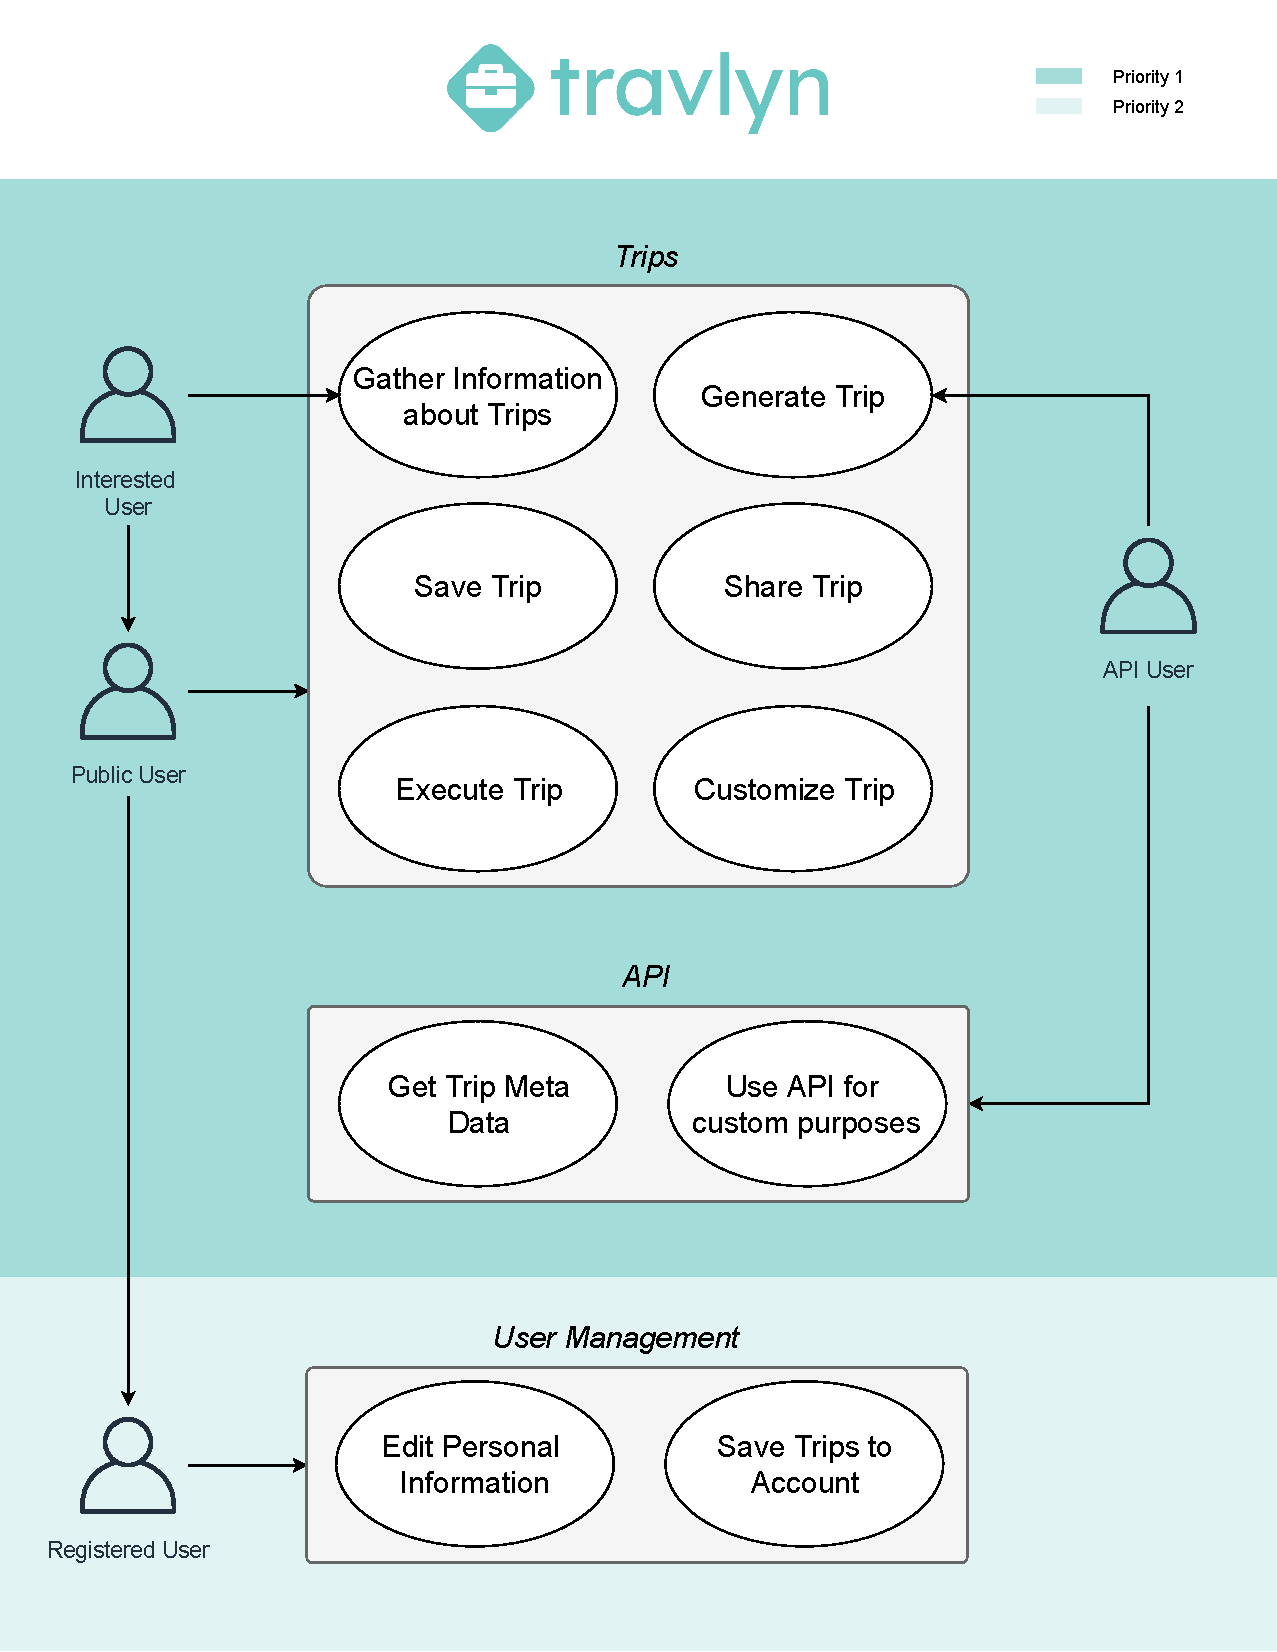
\includegraphics[width=1\textwidth]{images/UCD.pdf}
	\caption{Darstellung aller geplanten use cases mit den assoziierten Nutzerprofilen.}
	\label{fig:UCD}
\end{figure}

\newpage
